% ----- CONFIGURAÇÕES ----- %
\documentclass[12pt]{article}
\usepackage{graphicx} % imagens
\usepackage[brazil]{babel} % idioma
\usepackage{amsmath} % equações
\numberwithin{equation}{section} % numeração de equação numero-da-secao.numero-da-equacao
\usepackage{caption} % legenda em imagens e tabelas
\usepackage{subcaption} % legenda em subimagens e subtabelas
\newcommand{\source}[1]{\caption*{Fonte: {#1}} } % para adicionar fonte de imagens e tabelas
\usepackage{enumitem} % criação de listas
\usepackage{cite} % para citar seções, imagens...
\usepackage[hidelinks]{hyperref} % para ter itens (citação de seções, sumário...) clicáveis
\usepackage{indentfirst} % espaçamento do primeiro parágrafo
\setcounter{section}{-1} % começa as seções em 0
\usepackage{booktabs}
% --- ABNT --- %
% definindo fonte
\usepackage{fontspec}
\setmainfont{Times New Roman}
% tamanho da folha e margens
\usepackage[a4paper, left=3cm, top=3cm, right=2cm, bottom=2cm]{geometry}
% definindo tamanho para items e subitems
\usepackage{titlesec}
\titleformat{\section}{\normalfont\fontsize{16}{15}\bfseries}{\makebox[25pt][l]{\thesection}}{0pt}{}
\titleformat{\subsection}{\normalfont\fontsize{16}{15}\bfseries}{\makebox[25pt][l]{\thesubsection}}{0pt}{}
% para configurar alinhamento e espaçamento
\usepackage{setspace}
\usepackage{ragged2e}
\titlespacing*{\section}{0.75cm}{12pt}{12pt}
\titlespacing*{\subsection}{0.75cm}{12pt}{12pt}
\usepackage[alf,abnt-emphasize=bf]{abntex2cite} % bibliografia e citação no padrão ABNT

\usepackage{blindtext} % pacote para geração de texto aleatório, pode ser removido
\begin{document}
% ---- Renomeando títulos do sistema para português ---- %
\renewcommand*\contentsname{Sumário}
\renewcommand{\listfigurename}{Lista de Ilustrações}
\renewcommand{\listtablename}{Lista de Tabelas}
\renewcommand{\refname}{}
\onehalfspace % espaçamento entrelinhas 1.5
\justifying % alinhamento justificado
\setlength{\leftskip}{0.75cm} % corpo do texto a 0.75 cm da margem esquerda
\graphicspath{{./imagens/}} % pasta com imagens
\begin{titlepage}
    \begin{center}
        Escola Politécnica da Universidade de São Paulo\\
        Departamento de Engenharia X \\ Código - Disciplina\\

        \vspace{1.5cm}
        \includegraphics[width=0.4\textwidth]{Poli.png}
        
        \vspace*{1.5cm}
        \fontsize{18}{15}\textbf{TÍTULO}
        
        \vspace*{1.5cm}
        Prof. Dr. X

        \vspace*{1.5cm}
        \begin{tabular}{c c}
	        Nome & NUSP \\
            Nome & NUSP \\
            Nome & NUSP \\
            Nome & NUSP \\
            Nome & NUSP
        \end{tabular}
        
        \vspace*{\fill}
        {São Paulo\\
        Mês de 2024}
    \end{center}
\end{titlepage}
\newpage\textit{\textbf{Resumo: }até 250 palavras}

\textit{Palavras-chave: 3 palavras}
\newpage\textit{\textbf{Abstract: }maximum of 250 words}

\textit{Key-words: 3 words}
\newpage\listoffigures
\newpage\listoftables
\newpage\tableofcontents
\newpage\section{INTRODUÇÃO} \label{sec:intro}
\blindtext\cite{exemploArtigo}
\blindtext\cite{exemploLivro}
\blindtext\cite{exemploWeb}
\newpage\section{TITULO DA SECAO}\label{sec:conteudo1}
Além de citar referência bibliográfica com \cite{exemploArtigo}, você pode referenciar seções do relatório \autoref{sec:conteudo3} e \autoref{subsec:conteudo1}, figuras \autoref{fig:variasImagens} e \autoref{fig:poli3}, tabelas \autoref{tab:tabela} e equações \autoref{eq:relatividade}.

Exemplo de tabela:
\begin{table}[h!]
    \centering
    \caption{Tabela de exemplo}
    \begin{tabular}{cccc}
        \toprule
        \textbf{Item} & \textbf{Caracteristica 1} & \textbf{Caracteristica 2} & \textbf{Caracterista 3}\\
        \midrule
        x1 & y1 & z1 & w1\\
        x2 & y2 & z2 & w2\\
        \bottomrule
    \end{tabular}
    \label{tab:tabela}
\end{table}

Exemplo de imagem:
\begin{figure}[h!]
    \centering
    \caption{Imagem de exemplo}
    \includegraphics[width=0.5\textwidth]{imagens/Poli.png}
    \label{fig:poli}
    \source{\cite{exemploLivro}}
\end{figure}
Exemplo de equação:
\begin{equation}
    E = mc^2
    \label{eq:relatividade}
\end{equation}
Onde, \begin{itemize}
    \item $E$ é energia
    \item $m$ é massa
    \item $c=3\cdot10^3$ é a velocidade da luz no vácuo
\end{itemize}
\newpage Exemplo de multiplas imagens:
\begin{figure}[h!]
    \caption{Exemplo com varias imagens}
    \begin{subfigure} {0.5\textwidth}
        \includegraphics[width=0.9\textwidth]{imagens/Poli.png}
        \caption{Primeira imagem}
        \label{fig:poli1}
    \end{subfigure}
    \begin{subfigure}{0.5\textwidth}
        \includegraphics[width=0.9\textwidth]{imagens/Poli.png}
        \caption{Segunda imagem}
        \label{fig:poli2}
    \end{subfigure}
    \begin{subfigure}{0.5\textwidth}
        \includegraphics[width=0.9\textwidth]{imagens/Poli.png}
        \caption{Terceira imagem}
        \label{fig:poli3}
    \end{subfigure}
    \label{fig:variasImagens}
    \source{Autor}
\end{figure}
\subsection{Titulo da Subsecao}\label{subsec:conteudo1}
\blindtext

\noindent\textbf{\textit{Titulo da subsubsecao 1}}

\blindtext
\newpage\section{TITULO DA SECAO}\label{sec:conteudo2}
\blindtext
\subsection{Titulo da Subsecao}\label{subsec:conteudo2}
\blindtext

\noindent\textbf{\textit{Titulo da subsubsecao 2}}

\blindtext
\newpage\section{TITULO DA SECAO}\label{sec:conteudo3}
\blindtext

\subsection{Titulo da Subsecao}\label{subsec:conteudo3}
\blindtext

\noindent\textbf{\textit{Titulo da subsubsecao 3}}

\blindtext
\newpage\section{CONSIDERAÇÕES FINAIS}
\blindtext\blindtext\blindtext
\newpage\section{REFERÊNCIAS}
\bibliography{bibliografia}
\end{document}
